\section{Chess}
\subsection{Piece movement}
When checking for legal moves, the rules of chess and each piece are used.

General rules include: 

1. Pieces can not move onto squares with pieces of the same colour. This is checked by creating a matrix of the board, which is divided into rows and columns, and checking if the destination square is empty or occupied by an opponent's piece.

2. Each player gets one turn, in which one piece can be moved. However, in certain edge cases, more than one piece may be moved.

Furthermore some pieces' movements require additional capabilities.

\subsubsection{Knight}
The knight moves in an L shape and is the only piece that can move past pieces by jumping over them.

\subsubsection{Pawn}
The pawn can usually only move one square forward; however, the pawn behaves uniquely in many different edge cases: 

1. The pawn can move either one or two squares forward (column direction) only from the pawn's starting position (row 7 and 2).

2. The pawn captures pieces one square diagonal in front of it, meaning it is the only piece that captures in a different pattreviewedern than it moves. 

3. En passant: The pawn may, in certain cases, perform an "en passant". An example of this can be seen in \cref{fig: En passant}. In order to check an en passant, we have to check the move history, because the move can only be made directly after the pawn has moved two squares forward. To perform an en passant check is therefore different compared to normal moves. 

\begin{figure} [H]
    \centering
    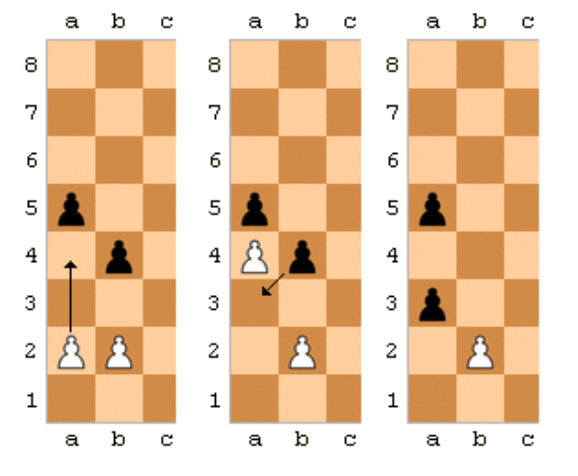
\includegraphics[width=0.6\linewidth]{Pictures/En_passant.png}
    \caption{En passant}
    \label{fig: En passant}
\end{figure}

4. Promotion: A promotion occurs when a pawn has moved to the furthest possible row. When this occurs, the pawn is traded for any other chosen piece by the player other than the king. Because the camera can not differentiate between different pieces, the program will always assume a queen promotion is made by the player.

\subsubsection{Rook}
The rook can move infinitely many squares in either the column direction or the row direction. The rook behaves uniquely when castling, which is explained later in subsection: Castling.

\subsubsection{Bishop}
The bishop can move infinitely many squares diagonally.

\subsubsection{Queen}
The queen moves as either a rook or a bishop, therefore, the move validator reuses the movement patterns of the bishop and rook and checks if either one is valid.

\subsubsection{King}
The king, like the pawn, seems basic in its functionality, but different edge cases make the king special. The king can move only one square each turn in any direction, however, the king cannot move into check, and is allowed to castle under certain conditions.

\subsubsection{Castling}
Castling is when the King moves two squares (instead of the usual one square) and the rook moves to the other side of the king (see \cref{fig: Castling} ). This can happen on either the king's side or the queen's side, where the rook moves an extra square if castling happens on the queen's side. This results in two pieces being moved in one turn and also requires that:

- The king has not moved previously.

- The king is not currently in check and has not been put in check previously.

- The rook on the side castling occurs has not moved either.

- The path between the king and rook is not occupied by other pieces, and is not under attack by the opponent's pieces, meaning the opponent's pieces can not move to the squares on the next turn.

In order to check all of the above conditions, a move history must be appended to after every turn, and the squares between the king and the rook must be checked if they are occupied by other pieces or under attack by the opponent's pieces.

\begin{figure} [H]
    \centering
    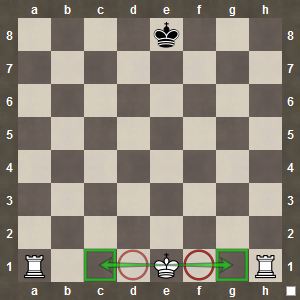
\includegraphics[width=0.5\linewidth]{Pictures/Possible-castling-moves.png}
    \caption{Castling}
    \label{fig: Castling}
\end{figure}

\subsection{Rules}

\subsubsection{Remis}
Remis (draw) can be achieved by 4 different scenarios:

1. 3-move rule: If the board has the exact same state 3 times in a game, it results in a draw. The move validator saves a copy of every board state and checks if the exact same board state has occured for a total of 3 times in a match.

2. 50-move rule: If the last 50 consecutive moves did not involve either a capture or the movement of a pawn, the game results in a draw. The move validator updates its half-move clock for every turn where  none of the moves above occured and resets if they do.

3. Insufficient material: If one side only has a king, and the other side only has a king, and either a horse or a bishop, the game also results in a draw, because a checkmate cannot occur with those pieces. The move validator checks if the only pieces left are the ones mentioned above by checking every square and counting what material is on the board.

4. Unable to move any pieces; however, the king is not in check. If no pieces can be moved on the given turn, the game also results in a draw. The move validator checks if there are any valid moves and if the king is in check.

\subsubsection{Check and checkmate}
A player is in check when the opponent can capture the king on the next turn, but only in check because the player has options to save the king. The player must either move the king out of check, obstruct the path of the attacking piece, or capture the attacking piece. The move validator checks if there is a valid move to the position the king is located for all of the opponent's pieces, and if there is, then the king must be in check. Then, if there is a valid move for the king which does not put him immediately in check again, the king is not in checkmate, and the game continues. 

Checkmate. If the king is in check, however, the king cannot be saved by either moving to a safe square, obstructing the path of the attacking piece, or capturing the attacking piece; the game ends, resulting in victory for the opponent. The move validator checks all possible options the player has, and if all of them still result in a check, then a checkmate has occurred.

%In this section, the central chessboard logic is reviewed in detail. In this project, computer vision is used to detect the player's moves. Previously, the inaccuracies of the implemented computer vision were discussed in depth. The chessboard logic class, along with a move-validator class, is central to this project. These classes are countermeasures, intended to increase the chances of interpreting a correct move from the computer vision. They are also crucial for detecting edge cases that require more than one piece to move at a time. They also check if the player is mated or if the game is tied (remis).

%Directly following a move from the player is a response from the robot. The robot calculates its move using Stockfish and communicates with the program through UCI (Universal Chess Interface). Stockfish is an AI that predicts the best move based on the configured depth and the previous moves. UCI is the language used to communicate through C++ with the Stockfish AI.

%**Detecting moves from the player as well as applying moves with the robot and the connection between the two are crucial elements in order to successfully complete a game of robot chess.**

\subsection{Stockfish UCI}

\subsubsection{Stockfish}
%Firstly a breif section on the stockfish AI. 
Stockfish uses an algorithm based on depth and the previous moves to determine the best possible move. The predetermined depth chosen by the user affects the abilities of the AI. Depth is a rough estimate of how far ahead Stockfish predicts. Theoretically, if the depth is defined by the user to be 10, then Stockfish predicts 10 half moves ahead (5 moves for white, and 5 for black). 

kilder: 
\href{https://www.chess.com/terms/stockfish-chess-engine}{Stockfish - Chess Engines - Chess.com} 
\href{https://www.chessprogramming.org/Depth}{Depth - Chessprogramming wiki} 

\subsubsection{Stockfish Class (UCI)}
The Stockfish UCI - Universal Chess Interface handles communication with and instantiates a local Stockfish. Stockfish uses all previously made moves to calculate the best next move. 
%Stockfish UCI - Universal Chess Interface, is the recommended way of communicating with Stockfish. UCI is a standard text-based protocol which uses various commands to communicate with Stockfish. The main part of the program flow follows this pattern. Write 'uci' and wait for 'uciok' to confirm two-way communication. Use 'isready' UCI command to ensure that the link between the program and AI has been made successfully. Read stockfish output until 'readyok' UCI command. Use the 'ucinewgame' command to initiate a new game. Now, the final and central commands that determine how the program communicates with Stockfish. Using 'position startpos moves ', Stockfish knows how to initialize the chessboard. Along with this command is a list of previous moves, which is what Stockfish uses to update its internal board state. Then, using 'go depth' UCI command, Stockfish starts searching for the best possible move. To end the communication and read the best move, we use a function in the UCI class which reads through the Stockfish output until the keyword 'bestmove' is found.

%**Using UCI, the depth of the Stockfish model can be configured to adjust difficulty. Because the UCI protocol requires a downloaded version of Stockfish, it becomes easier to use (no online communication etc.).**

%kilder:
%\href{https://official-stockfish.github.io/docs/stockfish-wiki/UCI-&-Commands.html\#uci}{Stockfish Docs} 

